\documentclass{standalone}

\usepackage{tikz}
\usepackage{tikz-3dplot}

\begin{document}
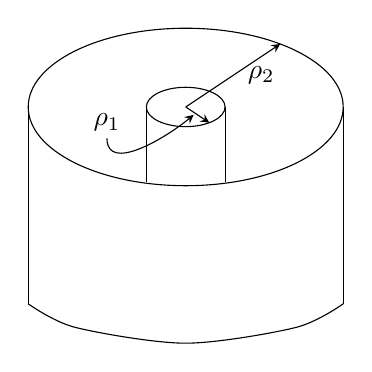
\begin{tikzpicture}
%\draw[thick,gray] (-3,-4) grid (3,3);
%\draw[thin,gray,step=0.2] (-3,-4) grid (3,3);

\draw(0,0) ellipse (2cm and 1cm);
\draw(0,0) ellipse (0.5cm and 0.25cm);

\draw(-2,0)--(-2,-2.5);
\draw(2,0)--(2,-2.5);

\draw(-0.5,0)--(-0.5,-0.95);
\draw(0.5,0)--(0.5,-0.95);

\draw[-stealth](0,0)--(0.3,-0.2);
\draw[-stealth](0,0)--(1.2,0.8) node[pos=0.8,below]{$\rho_2$};
\node at (-1,-0.2){$\rho_1$};
\draw[stealth-] (0.1,-0.1) to [out=220,in=-90] (-1,-0.4);

\draw plot[smooth] coordinates {(-2,-2.5) (-1.4,-2.8) (0,-3)  (1.4,-2.8) (2,-2.5)};
\end{tikzpicture}
\end{document} 
